\documentclass[a4paper, 10pt]{ctexart} %中文支持
\usepackage{float}              %防止浮动元素浮动
\usepackage{rotating}           %旋转图片
\usepackage{amsfonts}           %对某一些字体之支持
\usepackage{mathrsfs}           %mathscr e.g.
\usepackage[]{amsmath}          %数学公式
\usepackage{amsthm}             %定义, 定理, 证明, 例子环境的支持
%使用方法:
%\newtheorem{environment name}{caption}
%比如 \newtheorem{example}{这是例子}
%效果 \begin{example} xxx \end{example} -> 这是例子 1 xxx
%proof就不需要了
\usepackage{graphicx}           %插入图片
\usepackage[left=1.25in,right=1.25in,top=1in,bottom=1in]{geometry}   %用来排版的
\usepackage{color}            %给部分文本上色的
\usepackage{algorithm}          %写伪代码的
%\usepackage{algorithmic}       %同上
\usepackage{algorithmicx}
\usepackage{algpseudocode}
\usepackage{minted}
\usepackage{amssymb}            %用来加入一些数学符号, 比如说 $\varnothing$
\usepackage{titlesec}
\usepackage{fontspec}           %不知道用来干嘛的
\usepackage{hyperref}           %生成可跳转的书签
% -------------------------------
\setmonofont{Ubuntu Mono}       %?
\usemintedstyle{custommanni}    %设置minted插入代码的风格
\titleformat*{\section}{\huge\bfseries}             %管理title的字体和大小
\titleformat*{\subsection}{\Large\bfseries}         %bfseries就是默认的字体.
\titleformat*{\subsubsection}{\large\bfseries}
% -------------------------------
\newtheorem{theorem}{Theorem}
\newtheorem{example}{Example}
\newtheorem{definition}{Definition}
\newtheorem{lemma}{Lemma}
\newtheorem{remark}{Remark}
\newtheorem{corollary}{Comment}
\newtheorem{proposition}{Proposition}
\pagestyle{plain}
\title{chapter 9: String matching}
\author{You \and Me}
\date{date: Yesterday}

\begin{document}
\maketitle
\tableofcontents
\newpage

\section{Let us begin}
这里我并没有非常考虑读者的感受...

这里我们说, 哎, 真的, 我没什么时间了, 
总之我想快速地将这个东西飞完. 

我们说, 字符串匹配有什么要讲的呢? 
实际上就是面对这个 string matching 问题, 提出
各种各样的算法.
我们可以list a list: 
\begin{enumerate}
    \item 朴素匹配算法
    \item Rabin-Karp 算法
    \item finite automata 
    \item KMP 
    \item BST
\end{enumerate}

我们这里简单过一下, 
这里面的几个算法其实都比较有趣.
比如说 finite automata. 这个状态机
的概念是非常重要的. 有助于我们理解什么是
计算机. 

OK, 我们先是假设我们已经知道什么是
字符串匹配问题. 这里简单描述一下:
\begin{definition}[string matching problem]
We are given a text, denoted as $T$. Moreover, 
we are given a pattern, denoted as $P$. 
They are strings. We need to know that 
if there is pattern hidden in 
the text. 
\end{definition}
这里我们还没说清楚, 我们说一个优先字符串是什么? 
实际上是给定一个字母表 $\sum $, 而有限字符串
就是这个一个序列 $\left<a_{0}\cdots a_{n}\right> , a_{i} \in \sum_{}, i =0 , 1, \cdots , n$ 
这就是一个字符串了.
\begin{definition}[shift]
我们这样表示字符串的一部分. 我们从
0开始计数, 我们说 $T\left[ 0 \right]$ 
就是 $T$ 的初始的字母. $T\left[ 0 , 1, 2 ,3 \right]$ 就代表
这个 $T$ 中编号 $0 , 1, 2 , 3$ 组成的sub字符串.

而后我们说, string matching 问题
就是要找出一个shift $s$, 有 
\begin{align*}
    T[s,\cdots , s+m-1] = P[0,1,2,\cdots ,m]
\end{align*}
其中 $m$ 是这个东西的长度. 噢, 并且我们要找出这个
所有的 $s$
\end{definition}

好的, 说明完了, 
我们可以开始一个概述, 
我们从朴素方法开始. 

\subsection{朴素方法}
\paragraph{朴素方法} % (fold)
\label{par:朴素方法}
朴素方法没什么好说的, 这是因为,
额, 就是因为太简单了吧. 其实就是噢, 我, 
啊, 面对每一个shift, 我都恭敬地将
什么东西都比较了一遍. 

这里列举出时间复杂度. 
\begin{align*}
    T(n) =  \Theta \left( ( n - m + 1 ) m \right)
\end{align*}
只能说是明显.
% paragraph朴素方法 (end)

\subsection{Rabin-Karp algorithm}
\paragraph{Rabin-Karp algorithm} % (fold)
\label{par:Rabin-Karp algorithm}
这个是什么? 

就是介绍了一个指纹方法: 我们给定一个进制 $d$
然后给出一个string的指纹. 
\begin{align*}
    f\left( P\right) = 
    \sum_{i=0} ^{m-1}d^{m-i-1} \times p[i]
\end{align*}
就是将这个字母表映射到了一个正整数数组上面,
我们比较两个数字的速度要快得多, 利用这点
来加快比较过程. 

并且有一个递归方法进行指纹的计算, 我们设 $t_{s}$ 是 shift 为 $s$ 的时候
的 $T$ 的对应的 长度为 $m$ 的sub字符串的指纹值.
\begin{align*}
t_{s + 1} =\left[ t _{s} - T[s]\times d^{m-1} \right] \times d + T[s+m]
\end{align*}
Moreover, Rabin-Karp 算法还提倡使用 hash 方法进行一个优化, 
比如说当 $m$ 稍微长一点的时候, 就装不下了, 溢出了. 这个时候使用
hash 方法, 我也不是知道是不是这个名字, 
总之就是选取一个大于 $\left| \Sigma \right| $ 的质数. 
取模, 而后以模值作为指纹值. $q $ 为质数

同样的, 我们也有一个递归方法计算:
\begin{align*}
t _{s + 1} = \Big[\left[ t_{s} - T[s] \cdot c \right] \times d + T[s+m]  \Big]\mod q
\end{align*}
其中 $c$ 是 $d ^{m-1} \mod q$.  
这个公式非常重要!!!!! 至于这是哪里来的, 我超, 我哪里知道.

\begin{minted}[
    linenos
]{c++}
Rabin-Karp (T,P,d,p){
    int n = T.length;
    int m = P.length;
    int h = d^{m-1} mod q;
    p = 0;
    t_0 = 0;
    for (i=1 to m){ 
        p = (dp + P[i]) mod q;
        t_0 = (dt_0 + T[i]) mod q;
    }// this for loop is for preprocessing
    for (s=0 to n-m){ 
        if p==t_s {
            if P[0,...,m-1] == T[s,...,s+m-1]
                print s;
        }
        if (s < n-m)
            t_s+1 = blahblah;
    }// this for loop is for matching
}
\end{minted}

我们说, $s$ 有 $n-m+1$ 个取值, 
如果说 每一个 $s$ 都好巧不巧, 
tm的都有指纹相等的话, 这个东西就相当于
朴素匹配方法了. 

Worst case: 
\begin{align*}
    O \left( \left( n - m  + 1 \right) m\right)
\end{align*}
平均期望之下, 我们说, 发生suprious strike 的概率为 
\begin{align*}
    \frac{1}{q}
\end{align*}
那么说我们发生匹配的次数为 $\dfrac{n - m  + 1}{q}$ , 
乘起来
\begin{align*}
    \frac{n  - m+ 1 }{q} \times m = O\left( n - m + 1\right)
\end{align*}
% paragraphRabin-Karp algorithm (end)
\paragraph{finite automata} % (fold)
一个自动机, 是一个 5-tuple $ \left( Q ,q _{0} , A, \Sigma , \delta\right) $

\begin{definition}
定义如下:
\begin{enumerate}
    \item 
$ Q $ 是一个有限的集合, 其中元素称为是state.
    \item
$ q_{0} $ 是上面 $ Q $ 的一个元素, 称为初始状态
    \item 
$ A \subset Q $ 是一个子集, 称为accepting state 就是说, 当自动机走到这里的时候自动机就停止(或者干别的).
    \item 
$ \Sigma $ 是一个有限的集合, 其中元素称为字母, $ \Sigma $ 就是字母表.
    \item
$ \delta $ 是一个函数: $ Q \times \Sigma \to Q $ 
就是说, 对于
每一个state, 根据当前的input是 $ \sigma $ 
那么自动机将走到什么state. 这个函数成为是状态转移函数. 
(额, 我们可以联想一下马尔可夫链, 虽然差别很大, 但是那边也有一个状态转移函数)
\end{enumerate}
\end{definition}

\begin{figure}[]
    \centering
    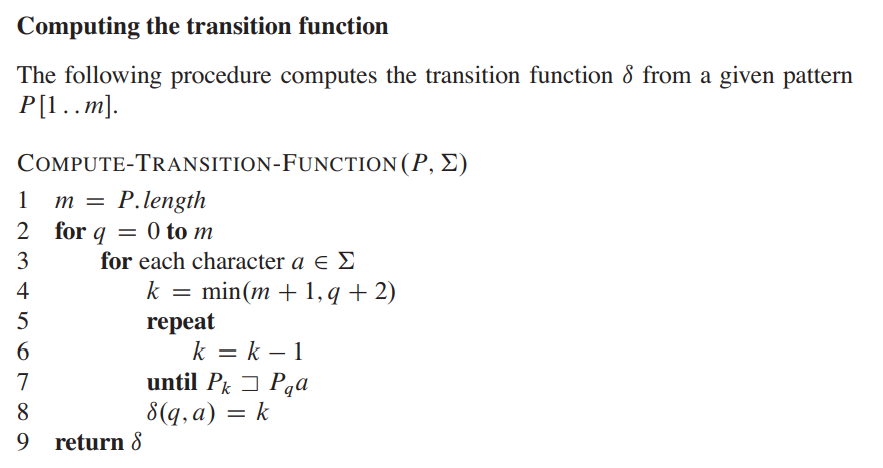
\includegraphics[scale = 0.5]{sm1.png}
    \caption{state transition function}
    \label{fig:sm1}
\end{figure} 
Figure~\ref{fig:sm1} 展示了一个状态转移函数的计算. 我们进行一点点分析.
$$ \delta (q, x)  =\sigma (P [0,q] ' x' )  = \max \{ k : P[0,k] \text{是} P[0,q] + \{x\} \text{的後綴}\} $$
\begin{itemize}
    \item 
line:2 从q=0开始, 相当于从矩阵第一行开始. 
    \item 
line:3 对于每一个a
    \item
line:4 $ k=\min\{m+1,q+2\} $这是因为 state 不会大于这两个前者是因为, 这种情况下匹配已经完成. q+2 是因为这个长度已经超过了当前的长度. 
    \item
line:7 直到当前匹配的后缀和P的前缀 P$_{k}$相同. 
\end{itemize}
The muching time that finite automata proceed along the Text is 
pretty good: $O \left(n\right)$. 
But the running that state transition requires is that 
$O\left( \left| \Sigma \right| m\right)$
% paragraph (end)

\subsection{KMP algorithm}
\paragraph{KMP} % (fold)
\label{par:KMP}
We follow ppt here.

The $\pi\left[ k \right]$ value is 
actually 
the length the longest common
prefix and suffix.

The while loop in the algorithm is 
a way to efficiently lower the 
value of k.  Figure~\ref{fig:sm2} shows a
example of how the 
pi array is worked out. And Figure~\ref{fig:sm3} 
is the code that calculates the 
pi array.
\begin{figure}[]
    \centering
    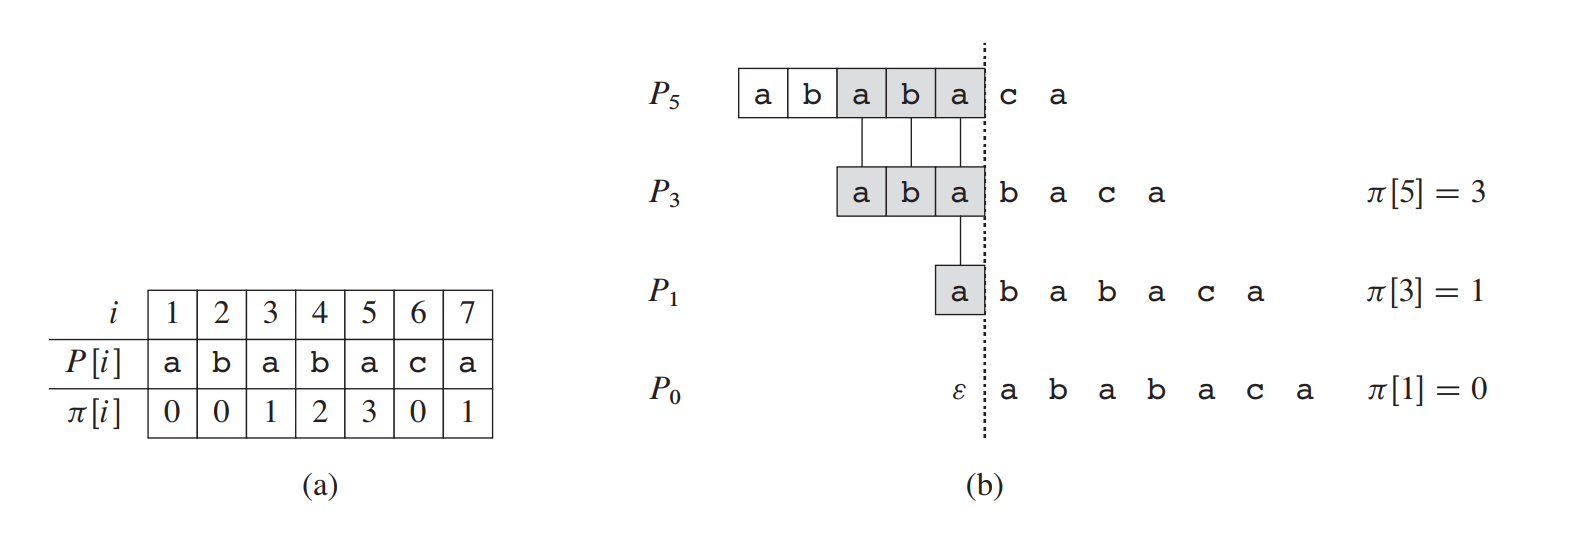
\includegraphics[scale  = 0.4]{sm2.png}
    \caption{pi array}
    \label{fig:sm2}
\end{figure}
\begin{figure}[]
    \centering
    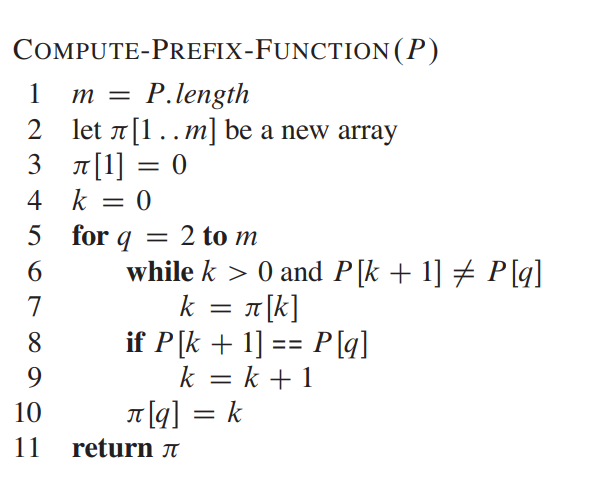
\includegraphics[scale = 0.5]{sm3.png}
    \caption{code}
    \label{fig:sm3}
\end{figure}
\begin{figure}[]
    \centering
    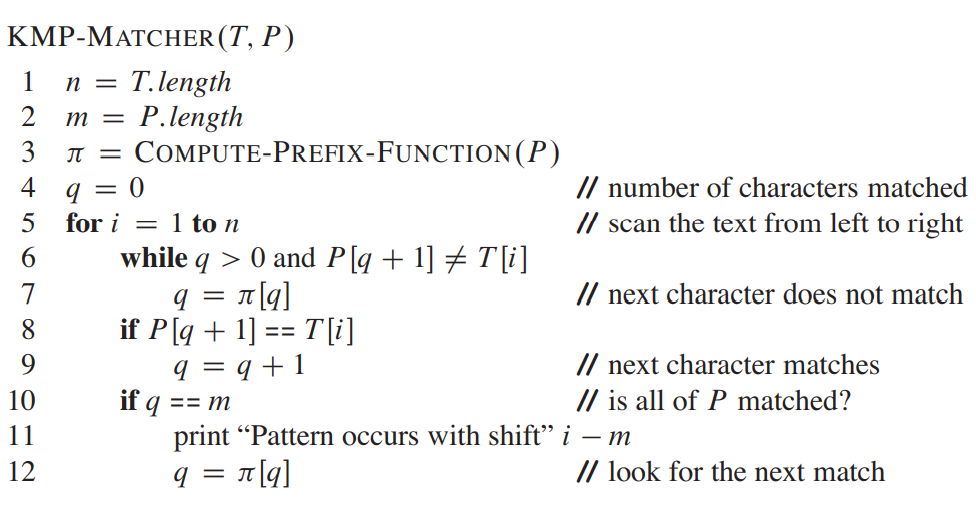
\includegraphics[scale = 0.5]{sm4.png}
    \caption{code of matcher}
    \label{fig:sm4}
\end{figure}

And then Figure~\ref{fig:sm4} is the code of 
how matcher works. 

Finally, without any proof, the ppt 
tells us that 
the worst case running time is 
$O\left( n  +m\right)$. 
Where we need $O\left(m\right)$ time to 
compute the $\pi$ array. 
% paragraphKMP (end)
\end{document}